% \VignetteIndexEntry{The otsad Package: Online Time-Series Anomaly Detectors}
% \VignetteDepends{otsad}
% \VignetteKeywords{otsad}
% \VignetteKeywords{anomaly time serie}
% \VignettePackage{otsad}
%\VignetteCompiler{knitr}
%\VignetteEngine{knitr::knitr}

\documentclass[a4paper]{article}\usepackage[]{graphicx}\usepackage[]{color}
%% maxwidth is the original width if it is less than linewidth
%% otherwise use linewidth (to make sure the graphics do not exceed the margin)
\makeatletter
\def\maxwidth{ %
  \ifdim\Gin@nat@width>\linewidth
    \linewidth
  \else
    \Gin@nat@width
  \fi
}
\makeatother

\definecolor{fgcolor}{rgb}{0.345, 0.345, 0.345}
\newcommand{\hlnum}[1]{\textcolor[rgb]{0.686,0.059,0.569}{#1}}%
\newcommand{\hlstr}[1]{\textcolor[rgb]{0.192,0.494,0.8}{#1}}%
\newcommand{\hlcom}[1]{\textcolor[rgb]{0.678,0.584,0.686}{\textit{#1}}}%
\newcommand{\hlopt}[1]{\textcolor[rgb]{0,0,0}{#1}}%
\newcommand{\hlstd}[1]{\textcolor[rgb]{0.345,0.345,0.345}{#1}}%
\newcommand{\hlkwa}[1]{\textcolor[rgb]{0.161,0.373,0.58}{\textbf{#1}}}%
\newcommand{\hlkwb}[1]{\textcolor[rgb]{0.69,0.353,0.396}{#1}}%
\newcommand{\hlkwc}[1]{\textcolor[rgb]{0.333,0.667,0.333}{#1}}%
\newcommand{\hlkwd}[1]{\textcolor[rgb]{0.737,0.353,0.396}{\textbf{#1}}}%
\let\hlipl\hlkwb

\usepackage{framed}
\makeatletter
\newenvironment{kframe}{%
 \def\at@end@of@kframe{}%
 \ifinner\ifhmode%
  \def\at@end@of@kframe{\end{minipage}}%
  \begin{minipage}{\columnwidth}%
 \fi\fi%
 \def\FrameCommand##1{\hskip\@totalleftmargin \hskip-\fboxsep
 \colorbox{shadecolor}{##1}\hskip-\fboxsep
     % There is no \\@totalrightmargin, so:
     \hskip-\linewidth \hskip-\@totalleftmargin \hskip\columnwidth}%
 \MakeFramed {\advance\hsize-\width
   \@totalleftmargin\z@ \linewidth\hsize
   \@setminipage}}%
 {\par\unskip\endMakeFramed%
 \at@end@of@kframe}
\makeatother

\definecolor{shadecolor}{rgb}{.97, .97, .97}
\definecolor{messagecolor}{rgb}{0, 0, 0}
\definecolor{warningcolor}{rgb}{1, 0, 1}
\definecolor{errorcolor}{rgb}{1, 0, 0}
\newenvironment{knitrout}{}{} % an empty environment to be redefined in TeX

\usepackage{alltt}
\usepackage[utf8]{inputenc}
\usepackage[T1]{fontenc}
\usepackage{amsmath,amssymb,array}
\usepackage{booktabs}

% Size of the layout
\usepackage[a4paper, total={160mm, 247mm}]{geometry}

%% load any required packages here

\usepackage{color}
\usepackage{stmaryrd}
\usepackage{url}
\usepackage[numbers,sectionbib]{natbib}

\usepackage{authblk}
\usepackage{epstopdf}
\IfFileExists{upquote.sty}{\usepackage{upquote}}{}
\begin{document}

\providecommand{\pkg}[1]{\textbf{#1}}
\providecommand{\CRANpkg}[1]{\textbf{#1}}
\providecommand{\code}[1]{\texttt{#1}}
\providecommand{\file}[1]{\texttt{'#1'}}

\title{The \pkg{otsad} Package:\\ Online Time-Series Anomaly Detectors}

%\author{Alaiñe Iturria}

\author[1,2]{Alaiñe Iturria}
\author[2]{Jacinto Carraso}
\author[2]{Francisco Herrera}
\author[1]{Santi Charramendieta}
\author[1]{Karmele Intxausti}

\affil[1]{IK4-Ikerlan, Big Data Architectures Team, Paseo J.Mª Arizmediarrieta, 2, 20500 Arrasate-Mondragon. Spain}
\affil[2]{Department of Computer Science and Artificial Intelligence, University of Granada, Granada, 18071, Spain}


\date{}

\maketitle

\definecolor{highlight}{rgb}{0,0,0}


\abstract{
Anomalies in time-series data give essential and often actionable information to be extracted from critical situations. Although this field has been widely studied, due to the continuous evolution of technology, new challenges arise that require further improvement and evolution of anomaly detection techniques. In this paper we present the \pkg{ostad} package that implements five of the most recent detection algorithms capable of dealing with various challenges, such as online and non-stationary time-series anomaly detection.
}

\section{Introduction}

Anomalies in time-series data give essential and often actionable information to be extracted for critical situations. This is an important task in many domains such as fault detection in manufacture, intrusion detection in cyber security or fraud detection in banks.

Anomaly detection is a wide field that has been studied for years. Chandola et al. \cite{Chandola}, Hodge et al. \cite{Hodge} and Zhang et al. \cite{Zhang} provide a comprehensive overview of anomaly detection techniques. The detection of anomalies involves the identification of patterns in the data that differ from expected behavior. In the classical literature the anomaly detection methods can be broadly categorized in six families: classification-based, clustering-based, nearest neighbors-based, statistics, information-theoretic based and spectral techniques.

Due to the evolution of new technologies, the amount of data is increasing and it is collected faster. For this reason, detection techniques must face new challenges such as an increase in the amount of data and online processing capacity. As opposed to classic techniques, online time-series anomaly detection techniques do not have the complete data set to work with and must take time into account. In recent years, most of the work has focused on the evolution of predictive and moving window-based techniques  \cite{a3e0f1cf080343d98cae7430cd6e43c4}.

In R statistical software, there are few packages available from \emph{Comprehensive R Archive Network (CRAN)} to address the problem of time-series anomaly detection. The first and most popular is the \CRANpkg{tsoutliers} package. There is also the \CRANpkg{qicharts} package that implements basic control chart algorithms. Finally, another package that is becoming increasingly popular is \pkg{Twitter's AnomalyDetection} package (only available on GitHub). One of the main disadvantages of these three packages is that the implemented algorithms are not suitable to work online. In addition to the aforementioned, there are two other packages, \CRANpkg{SmartSifter} and \CRANpkg{EnergyOnlineCPM} available for online time-series anomaly detection.

In conclusion, there are only a few packages for online anomaly detection available in CRAN. For this reason, we propose the \pkg{otsad} pacakge that implements 5 recent and powerful algorithms for the detection of anomalies in univariate time-series able to work online.

In the following section \ref{sec:online} we briefly introduce what online time-series anomaly detection is all about. In in the following section \ref{sec:package} we show how to use the \pkg{otsad} package using two easy examples. Finally, in section \ref{sec:summary}, we present an overview of this work.

\section{Online anomaly detection in time-series}\label{sec:online}

The detection of anomalies in online time-series is a difficult task because it must be able to consider the time (or the position of each observation) and it does not have entire dataset available. As mentioned earlier, in the last few years it is focusing on the evolution of predictive-based and moving window-based detection techniques.

Predictive techniques are models in which the parameters or components of the model are modified as new data arrive to capture better normal data trends. They calculate if a value is anomalous based on the dissimilarity or the error obtained between the observation and its prediction. On the other hand, techniques based on moving windows are are commonly used to improve distance-based techniques. Distance calculation is an expensive process and proportional to the number of observations to be considered, the use of moving windows allows reducing the set of observations to be considered maintaining the most recent subset of data.

Another major challenge with the introduction of online processing is that time-series can be stationary and non-stationary. A time-series is said to be stationary when the mean and variance remain constant over time. In addition, they must be neither seasonal nor trendy. Most statistical or predictive techniques assume that time-series are stationary, when in most real cases they never are. It is true that there are techniques to turn a non-stationary time-series into a stationary one, however, this is not a simple task and there are cases this can not be done stationary.

With the \pkg{ostad} package we provide five algorithms that address these three challenges. All algorithms can be used online. Furthermore, two of the five algorithms can be used in stationary environments and the other three in non-stationary environments. Finally, three of the techniques are based on predictive methods while the other two use moving windows based on techniques.

\section{The \pkg{otsad} package}\label{sec:package}

The package provided implements, documents, explains and provides references for a set of detectors listed below. In our opinion, this is the first review and package for R that develops a set of current and powerful anomaly detectors for the online detection of anomalies in time-series.

The \pkg{otsad} package implements five anomaly detection algorithms: PEWMA, SD-EWMA, TSSD-EWMA, KNNN-CAD and KNN-LDCD. The first three algorithms belong to prediction-based techniques and the last two belong to window-based techniques. Figure \ref{fig:features} shows a table with the most important characteristics of each algorithm.

\begin{itemize}
\item \emph{PEWMA} or \emph{Probabilistic reasoning for streaming anomaly detection} \cite{pewma}. Probabilistic reasoning for streaming anomaly detection. This algorithm is a probabilistic method of EWMA which dynamically adjusts the parameterization based on the probability of the given observation. This method produces dynamic, data-driven anomaly thresholds which are robust to abrupt transient changes, yet quickly adjust to long-term distributional shifts.

\item \emph{SD-EWMA} or \emph{Shift-Detection based on EWMA} \cite{Raza}. This algorithm is a novel method for covariate shift-detection tests for univariate time-series. It works in an online mode and it uses an exponentially weighted moving average (EWMA) model based control chart to detect the covariate shift-point in stationary time-series.

\item \emph{TSSD-EWMA} or \emph{Two-Stage Shift-Detection based on EWMA} \cite{Raza}. This algorithm is a novel method for covariate shift-detection tests based on a two-stage structure for univariate time-series. It works in an online mode and it uses an exponentially weighted moving average (EWMA) model based control chart to detect the covariate shift-point in non-stationary time-series. This algorithm works in two phases. In the first phase, it detects anomalies using the SD-EWMA algorithm. In the second phase, it checks the veracity of the anomalies using the Kolmogorov-Simirnov test to reduce false alarms.

\item \emph{KNN-CAD} or \emph{Conformal k-NN Anomaly Detector} \cite{2016arXiv160804585B}. This algorithm is a model-free anomaly detection method for univariate time-series which adapts itself to non-stationarity in the data stream and provides probabilistic abnormality scores based on the conformal prediction paradigm.

\item \emph{KNN-LDCD} or \emph{KNN - Lazy Drifting Conformal Detector}  \cite{2017arXiv170603412I}. This algorithm is a variant of the KNN-CAD algorithm. The difference between the two, lies in the calculation of the measure of dissimilarity and in the calculation of the conformity function. The KNN-CAD and KNN-LDCD algorithms use both distance-based techniques, KNN, and statistical techniques to determine the degree of anomaly.
\end{itemize}

\begin{figure}[htbp]
\centering
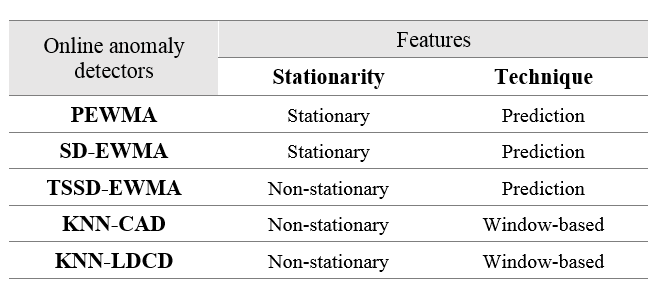
\includegraphics[width=0.7\linewidth]{features.PNG}
\caption{Features of the anomaly detectors available in the \pkg{otsad} package.}
\label{fig:features}
\end{figure}

Each of these algorithms has been implemented to work in two different scenarios. On the one hand, classical processing, used when the complete data set (train and test) is available. On the other hand, the incremental processing used when no data set is available. It allows you to calculate the abnormality of the new observation(s) with the parameters updated in the last run performed.

The rest of the section is organized as follows. Section \ref{sec:installation} is devoted to the installation process. In section \ref{sec:documentation} we present the documentation. Finally, in Section \ref{sec:example}, we show how to use the algorithms using two simple examples.

\subsection{Installation}\label{sec:installation}

The \pkg{otsad} package is available at GitHub repository, so it can be downloaded and installed directly from the R command line by typing:

\begin{knitrout}
\definecolor{shadecolor}{rgb}{0.969, 0.969, 0.969}\color{fgcolor}\begin{kframe}
\begin{alltt}
\hlkwd{install.packages}\hlstd{(}\hlstr{"devtools"}\hlstd{)}
\hlstd{devtools}\hlopt{::}\hlkwd{install_github}\hlstd{(}\hlstr{"alaineiturria/otsad"}\hlstd{)}
\end{alltt}
\end{kframe}
\end{knitrout}

To easily access all the package’s functions, it must be attached in the usual way:

\begin{knitrout}
\definecolor{shadecolor}{rgb}{0.969, 0.969, 0.969}\color{fgcolor}\begin{kframe}
\begin{alltt}
\hlkwd{library}\hlstd{(otsad)}
\end{alltt}
\end{kframe}
\end{knitrout}

\subsection{Documentation}\label{sec:documentation}

Considering that this vignette provides the user with an overview of the \pkg{otsad} package, it is also important to have access to the specific information of each of the available algorithms. This information can be checked in the documentation page corresponding to each algorithm. In all cases, the documentation has the same structure, consisting of the following sections (see Figure \ref{fig:documentation} for an example):

\begin{itemize}
\item A \emph{description} section, which gives a brief description of what the algorithm consists of (like those given in Section \ref{sec:package}).
\item A \emph{usage} section, where an overview of the function with the available parameters is given.
\item An \emph{arguments} section, where each of the input parameters is described.
\item A \emph{details} section, which provides the user with more details on the algorithm, conditions and recommendations on the values that can be taken by each of the input parameters.
\item A \emph{value} section, where the output parameters of the function are described.
\item A \emph{references} section that points to the original contribution where the detector(s) was proposed, where further details, motivations or contextualization can be found.
\item An \emph{examples} section, where one or more examples of the use of the functions are shown.
\end{itemize}

As usual in R, the documentation pages for each function can be loaded from the command line with the commands \code{?} or \code{help}:

\begin{knitrout}
\definecolor{shadecolor}{rgb}{0.969, 0.969, 0.969}\color{fgcolor}\begin{kframe}
\begin{alltt}
\hlopt{?}\hlstd{CpSdEwma}
\hlkwd{help}\hlstd{(CpSdEwma)}
\end{alltt}
\end{kframe}
\end{knitrout}

In addition, a user manual is available in the github repository of the  \pkg{otsad} package, which contains the complete documentation of the package and its functions.

\begin{figure}[htbp]
\centering
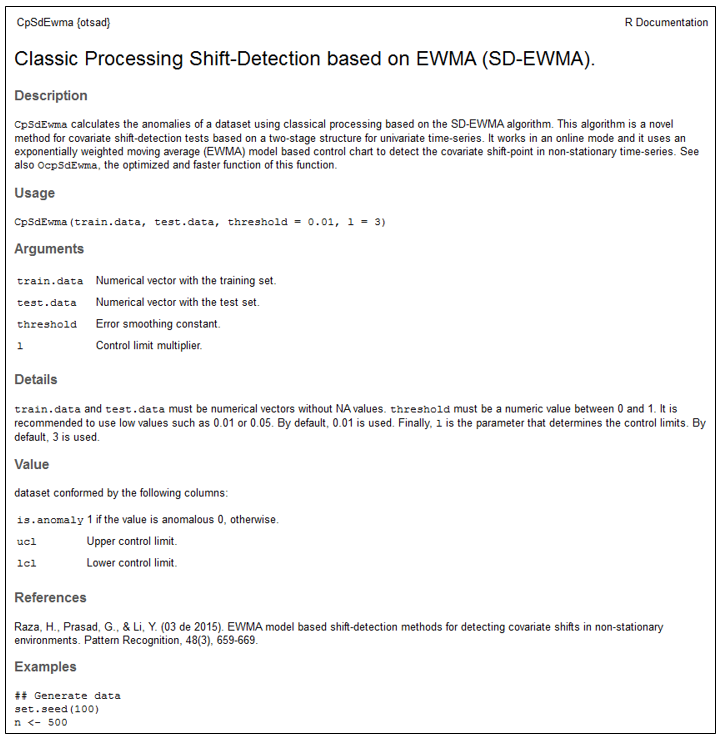
\includegraphics[width=0.5\linewidth]{documentationExample.png}
\caption{Extract from CpSdEwma detectors documentation page, showing the highlighted above aspects.}
\label{fig:documentation}
\end{figure}

\newpage

\subsection{Use example}\label{sec:example}

Here is an example of how to solve a simple problem. The example will be made with the SD-EWMA algorithm. The data has been generated as follows:

\begin{knitrout}
\definecolor{shadecolor}{rgb}{0.969, 0.969, 0.969}\color{fgcolor}\begin{kframe}
\begin{alltt}
\hlcom{## Generate data}
\hlkwd{set.seed}\hlstd{(}\hlnum{100}\hlstd{)}
\hlstd{n} \hlkwb{<-} \hlnum{500}
\hlstd{x} \hlkwb{<-} \hlkwd{sample}\hlstd{(}\hlnum{1}\hlopt{:}\hlnum{100}\hlstd{, n,} \hlkwc{replace} \hlstd{=} \hlnum{TRUE}\hlstd{)}
\hlstd{x[}\hlnum{70}\hlopt{:}\hlnum{90}\hlstd{]} \hlkwb{<-} \hlkwd{sample}\hlstd{(}\hlnum{110}\hlopt{:}\hlnum{115}\hlstd{,} \hlnum{21}\hlstd{,} \hlkwc{replace} \hlstd{=} \hlnum{TRUE}\hlstd{)} \hlcom{# distributional shift}
\hlstd{x[}\hlnum{25}\hlstd{]} \hlkwb{<-} \hlnum{200} \hlcom{# abrupt transient anomaly}
\hlstd{x[}\hlnum{320}\hlstd{]} \hlkwb{<-} \hlnum{170} \hlcom{# abrupt transient anomaly}
\hlstd{df} \hlkwb{<-} \hlkwd{data.frame}\hlstd{(}\hlkwc{timestamp} \hlstd{=} \hlnum{1}\hlopt{:}\hlstd{n,} \hlkwc{value} \hlstd{= x)}
\end{alltt}
\end{kframe}
\end{knitrout}

We can visualize the time-series as in Figure \ref{fig:ts} by typing:
\begin{knitrout}
\definecolor{shadecolor}{rgb}{0.969, 0.969, 0.969}\color{fgcolor}\begin{kframe}
\begin{alltt}
\hlkwd{plot}\hlstd{(}\hlkwc{x} \hlstd{= df}\hlopt{$}\hlstd{timestamp,} \hlkwc{y} \hlstd{= df}\hlopt{$}\hlstd{value,} \hlkwc{type} \hlstd{=} \hlstr{"l"}\hlstd{,}
     \hlkwc{main} \hlstd{=} \hlstr{"Time-Serie"}\hlstd{,} \hlkwc{col} \hlstd{=} \hlstr{"blue"}\hlstd{,} \hlkwc{xlab} \hlstd{=} \hlstr{"Time"}\hlstd{,} \hlkwc{ylab} \hlstd{=} \hlstr{"Value"}\hlstd{)}
\end{alltt}
\end{kframe}
\end{knitrout}

\begin{figure}[htbp]
\centering
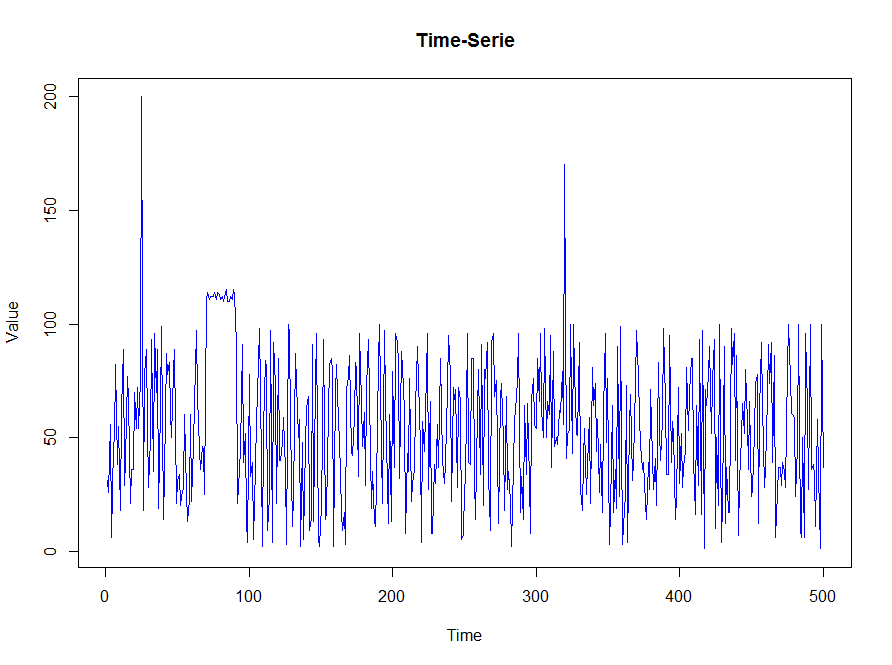
\includegraphics[width=0.5\linewidth]{timeSerie.PNG}
\caption{Our time-series visualization}
\label{fig:ts}
\end{figure}


The SD-EWMA algorithm is designed for stationary time-series. Therefore, we must first check that the time-series is stationary. To do this, we can display the acf and pacf graphics (Figure \ref{fig:acf}) by:

\begin{knitrout}
\definecolor{shadecolor}{rgb}{0.969, 0.969, 0.969}\color{fgcolor}\begin{kframe}
\begin{alltt}
\hlstd{forecast}\hlopt{::}\hlkwd{Acf}\hlstd{(}\hlkwd{ts}\hlstd{(df}\hlopt{$}\hlstd{value),} \hlkwc{main} \hlstd{=} \hlstr{"ACF"}\hlstd{,} \hlkwc{lag} \hlstd{=} \hlnum{20}\hlstd{)}
\hlstd{forecast}\hlopt{::}\hlkwd{Pacf}\hlstd{(}\hlkwd{ts}\hlstd{(df}\hlopt{$}\hlstd{value),} \hlkwc{main} \hlstd{=} \hlstr{"PACF"}\hlstd{,} \hlkwc{lag} \hlstd{=} \hlnum{20}\hlstd{)}
\end{alltt}
\end{kframe}
\end{knitrout}

\begin{figure}[htbp]
\centering
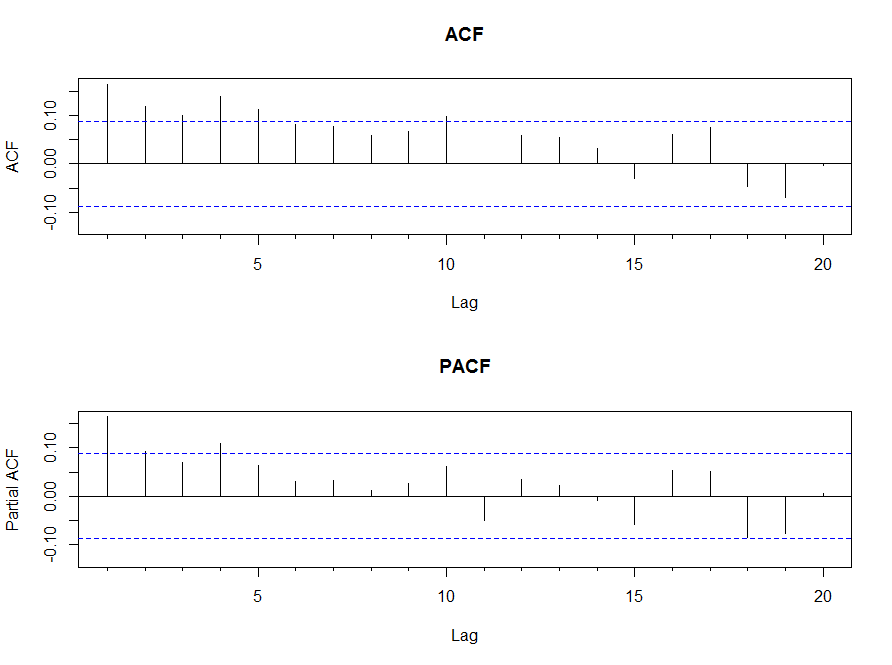
\includegraphics[width=0.5\linewidth]{acf.PNG}
\caption{ACF and PACF graphs}
\label{fig:acf}
\end{figure}

We can observe that since almost all the lags are within the limits, the time-series is stationary. In addition, we can use two statistical tests, adf test and kpss test. The tests also indicate that the time-series is stationary.

\begin{knitrout}
\definecolor{shadecolor}{rgb}{0.969, 0.969, 0.969}\color{fgcolor}\begin{kframe}
\begin{alltt}
\hlkwd{library}\hlstd{(tseries)}
\hlkwd{adf.test}\hlstd{(df}\hlopt{$}\hlstd{value,} \hlkwc{alternative} \hlstd{=} \hlstr{'stationary'}\hlstd{,} \hlkwc{k} \hlstd{=} \hlnum{0}\hlstd{)}
\hlkwd{kpss.test}\hlstd{(df}\hlopt{$}\hlstd{value)}
\end{alltt}
\end{kframe}
\end{knitrout}

On the recommendation of the algorithm authors, also indicated in the details section of this function, we set \code{threshold} to 0.01.One of the usual values for the $\sigma$ multiplier \code{l} is usually 3. Next, we apply the SD-EWMA anomaly detector, as the example is simple we use the classical processing algorithm. Note that the optimized algorithm could be used in the same way. Finally, we separate the training and test sets, using the first five values for training and the rest values for testing.

\begin{knitrout}
\definecolor{shadecolor}{rgb}{0.969, 0.969, 0.969}\color{fgcolor}\begin{kframe}
\begin{alltt}
\hlstd{train} \hlkwb{<-} \hlstd{df[}\hlnum{1}\hlopt{:}\hlnum{5}\hlstd{,}\hlstr{"value"}\hlstd{]}
\hlstd{test} \hlkwb{<-} \hlstd{df[}\hlnum{6}\hlopt{:}\hlstd{n,}\hlstr{"value"}\hlstd{]}
\hlstd{result} \hlkwb{<-} \hlkwd{CpSdEwma}\hlstd{(train, test,} \hlkwc{threshold} \hlstd{=} \hlnum{0.01}\hlstd{,} \hlkwc{l} \hlstd{=} \hlnum{3}\hlstd{)}
\end{alltt}
\end{kframe}
\end{knitrout}

If we print the results we can observe that the results are of data.frame type and have three columns: \emph{is.anomaly} indicating whether or not the test observation is anomalous and the columns \emph{ucl} and \emph{lcl} with the upper and lower control limits, used to determine whether or not the observation is anomalous.

\begin{knitrout}
\definecolor{shadecolor}{rgb}{0.969, 0.969, 0.969}\color{fgcolor}\begin{kframe}
\begin{alltt}
\hlkwd{head}\hlstd{(result,} \hlkwc{n} \hlstd{=} \hlnum{10}\hlstd{)}
\end{alltt}
\begin{verbatim}
##    is.anomaly        lcl      ucl
## 1       FALSE -16.718459 83.33762
## 2       FALSE -15.120715 84.87796
## 3       FALSE -12.127443 91.30896
## 4       FALSE -12.029491 90.89286
## 5       FALSE -10.427275 92.40430
## 6       FALSE -12.931167 90.31049
## 7       FALSE -10.756584 92.99798
## 8       FALSE  -7.669897 99.48715
## 9       FALSE  -9.332986 97.76851
## 10      FALSE  -9.501358 97.09333
\end{verbatim}
\end{kframe}
\end{knitrout}

Finally, we can see the results (Figure \ref{fig:result}) by writing the following code:

\begin{knitrout}
\definecolor{shadecolor}{rgb}{0.969, 0.969, 0.969}\color{fgcolor}\begin{kframe}
\begin{alltt}
\hlkwd{library}\hlstd{(ggplot2)}
\hlstd{res} \hlkwb{<-} \hlkwd{cbind}\hlstd{(df[}\hlnum{6}\hlopt{:}\hlstd{n,], result)}
\hlkwd{rownames}\hlstd{(res)} \hlkwb{<-} \hlnum{1}\hlopt{:}\hlkwd{length}\hlstd{(test)}

\hlkwd{ggplot}\hlstd{(res,} \hlkwd{aes}\hlstd{(timestamp, value))} \hlopt{+}
      \hlkwd{geom_line}\hlstd{(}\hlkwc{na.rm}\hlstd{=}\hlnum{TRUE}\hlstd{,} \hlkwc{color} \hlstd{=} \hlstr{"blue"}\hlstd{)} \hlopt{+}
      \hlkwd{ggtitle}\hlstd{(}\hlstr{"SD-EWMA Anomaly Detector"}\hlstd{)} \hlopt{+}
      \hlkwd{xlab}\hlstd{(}\hlstr{"Time"}\hlstd{)} \hlopt{+} \hlkwd{ylab}\hlstd{(}\hlstr{"Value"}\hlstd{)} \hlopt{+}
      \hlkwd{theme}\hlstd{(}\hlkwc{plot.title} \hlstd{=} \hlkwd{element_text}\hlstd{(}\hlkwc{lineheight}\hlstd{=}\hlnum{.8}\hlstd{,} \hlkwc{face}\hlstd{=}\hlstr{"bold"}\hlstd{,} \hlkwc{size} \hlstd{=} \hlnum{20}\hlstd{))} \hlopt{+}
      \hlkwd{theme}\hlstd{(}\hlkwc{text} \hlstd{=} \hlkwd{element_text}\hlstd{(}\hlkwc{size}\hlstd{=}\hlnum{18}\hlstd{))} \hlopt{+}
      \hlkwd{geom_point}\hlstd{(}\hlkwc{data} \hlstd{= res[res}\hlopt{$}\hlstd{is.anomaly} \hlopt{==} \hlnum{TRUE}\hlstd{,],}\hlkwd{aes}\hlstd{(}\hlkwc{colour} \hlstd{=} \hlkwd{factor}\hlstd{(is.anomaly)))} \hlopt{+}
      \hlkwd{theme}\hlstd{(}\hlkwc{legend.position}\hlstd{=}\hlstr{"none"}\hlstd{)}
\end{alltt}
\end{kframe}
\end{knitrout}

\begin{figure}[htbp]
\centering
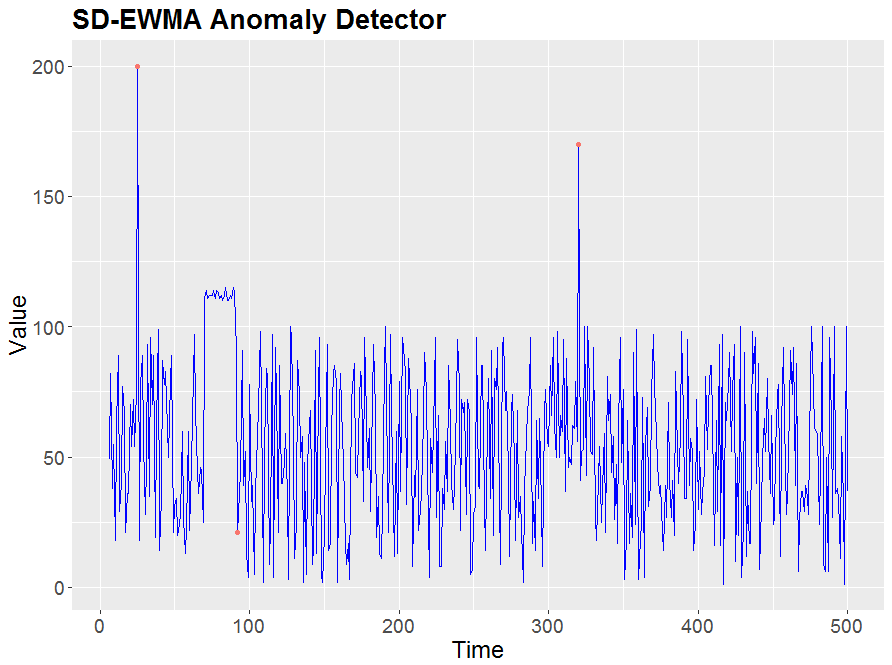
\includegraphics[width=0.5\linewidth]{sdEwmaresult.PNG}
\caption{Sd-Ewma Anomaly detector results}
\label{fig:result}
\end{figure}

In Figure \ref{fig:result} we can see that the detector has detected both abrupt transient anomalies well and the third one, distributional shift anomaly, a little late.

This example has used classical processing, but by using the incremental function we can simulate online processing as follows:

\begin{knitrout}
\definecolor{shadecolor}{rgb}{0.969, 0.969, 0.969}\color{fgcolor}\begin{kframe}
\begin{alltt}
\hlcom{## Initialize parameters for the loop}
\hlstd{last.res} \hlkwb{<-} \hlkwa{NULL}
\hlstd{res} \hlkwb{<-} \hlkwa{NULL}
\hlstd{nread} \hlkwb{<-} \hlnum{250}
\hlstd{numIter} \hlkwb{<-} \hlstd{n}\hlopt\hlstd{nread}
\hlstd{iter} \hlkwb{<-} \hlkwd{seq}\hlstd{(}\hlnum{1}\hlstd{, nread} \hlopt{*} \hlstd{numIter, nread)}

\hlcom{## Calculate anomalies}
\hlkwa{for}\hlstd{(i} \hlkwa{in} \hlstd{iter) \{}
  \hlcom{# read new data}
  \hlstd{newRow} \hlkwb{<-} \hlstd{df[i}\hlopt{:}\hlstd{(i} \hlopt{+} \hlstd{nread} \hlopt{-} \hlnum{1}\hlstd{),]}
  \hlcom{# calculate if it's an anomaly}
  \hlstd{last.res} \hlkwb{<-} \hlkwd{IpSdEwma}\hlstd{(}
    \hlkwc{data} \hlstd{= newRow}\hlopt{$}\hlstd{value,}
    \hlkwc{n.train} \hlstd{=} \hlnum{5}\hlstd{,}
    \hlkwc{threshold} \hlstd{=} \hlnum{0.01}\hlstd{,}
    \hlkwc{l} \hlstd{=} \hlnum{3}\hlstd{,}
    \hlkwc{last.res} \hlstd{= last.res}\hlopt{$}\hlstd{last.res}
  \hlstd{)}
  \hlcom{# prepare the result}
  \hlkwa{if}\hlstd{(}\hlopt{!}\hlkwd{is.null}\hlstd{(last.res}\hlopt{$}\hlstd{result))\{}
    \hlstd{res} \hlkwb{<-} \hlkwd{rbind}\hlstd{(res,} \hlkwd{cbind}\hlstd{(newRow[(nread} \hlopt{-} \hlkwd{nrow}\hlstd{(last.res}\hlopt{$}\hlstd{result)} \hlopt{+} \hlnum{1}\hlstd{)}\hlopt{:}\hlstd{nread,], last.res}\hlopt{$}\hlstd{result))}
  \hlstd{\}}
\hlstd{\}}
\end{alltt}
\end{kframe}
\end{knitrout}

In the same way we can view the results (Figure ref{fig:result2}) by writing:

\begin{knitrout}
\definecolor{shadecolor}{rgb}{0.969, 0.969, 0.969}\color{fgcolor}\begin{kframe}
\begin{alltt}
\hlkwd{library}\hlstd{(ggplot2)}

\hlkwd{ggplot}\hlstd{(res,} \hlkwd{aes}\hlstd{(timestamp, value))} \hlopt{+}
      \hlkwd{geom_line}\hlstd{(}\hlkwc{na.rm}\hlstd{=}\hlnum{TRUE}\hlstd{,} \hlkwc{color} \hlstd{=} \hlstr{"blue"}\hlstd{)} \hlopt{+}
      \hlkwd{ggtitle}\hlstd{(}\hlstr{"Online SD-EWMA Anomaly Detector"}\hlstd{)} \hlopt{+}
      \hlkwd{xlab}\hlstd{(}\hlstr{"Time"}\hlstd{)} \hlopt{+} \hlkwd{ylab}\hlstd{(}\hlstr{"Value"}\hlstd{)} \hlopt{+}
      \hlkwd{theme}\hlstd{(}\hlkwc{plot.title} \hlstd{=} \hlkwd{element_text}\hlstd{(}\hlkwc{lineheight}\hlstd{=}\hlnum{.8}\hlstd{,} \hlkwc{face}\hlstd{=}\hlstr{"bold"}\hlstd{,} \hlkwc{size} \hlstd{=} \hlnum{20}\hlstd{))} \hlopt{+}
      \hlkwd{theme}\hlstd{(}\hlkwc{text} \hlstd{=} \hlkwd{element_text}\hlstd{(}\hlkwc{size}\hlstd{=}\hlnum{18}\hlstd{))} \hlopt{+}
      \hlkwd{geom_point}\hlstd{(}\hlkwc{data} \hlstd{= res[res}\hlopt{$}\hlstd{is.anomaly} \hlopt{==} \hlnum{TRUE}\hlstd{,],}\hlkwd{aes}\hlstd{(}\hlkwc{colour} \hlstd{=} \hlkwd{factor}\hlstd{(is.anomaly)))} \hlopt{+}
      \hlkwd{theme}\hlstd{(}\hlkwc{legend.position}\hlstd{=}\hlstr{"none"}\hlstd{)}
\end{alltt}
\end{kframe}
\end{knitrout}

\begin{figure}[htbp]
\centering
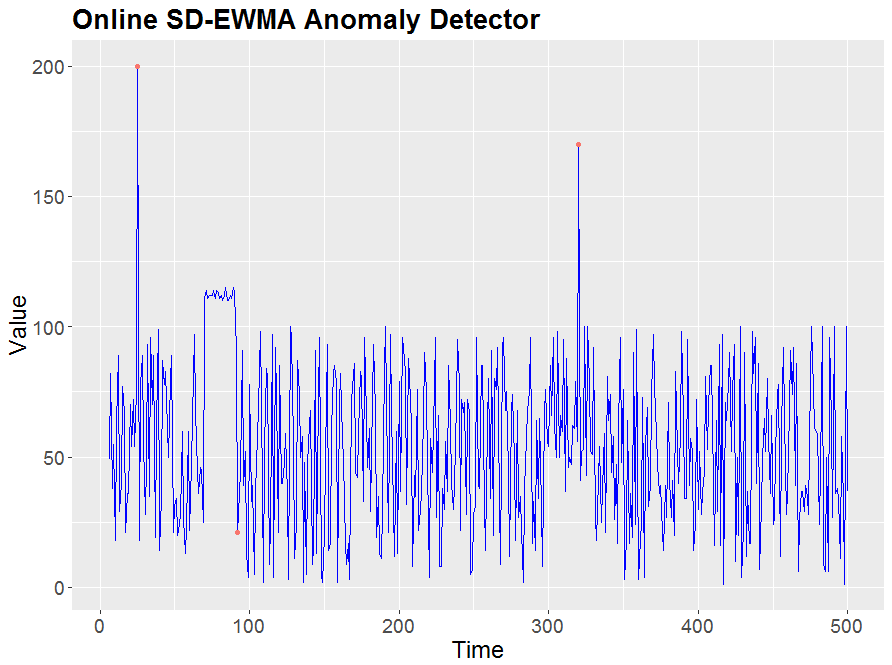
\includegraphics[width=0.5\linewidth]{onlineSdEwma.PNG}
\caption{Online Sd-Ewma Anomaly detector results}
\label{fig:result2}
\end{figure}

\section{Summary}\label{sec:summary}

In this vignette we introduce the \pkg{otsad} package, which implements five recent algorithms for online anomaly detection. In order to the context and motivation for this work we present the new challenges faced by time-series anomaly detection techniques with the introduction of the need for online processing. As explained in section \ref{sec:online}, the package proposes three algorithms based on the most recent prediction techniques (derived from EWMA) and two, based on moving window techniques (derived from KNN-CAD). Likewise, we cover the problem of the stationarity of time-series since two of the proposed algorithms have been designed to work in stationary environments and the other three can work in non-stationary environments. Finally, all algorithms can be used in two different scenarios: classical processing and incremental processing.

Regarding the future extensions of this package, there are several aspects that may be addressed in the future  (e.g., functions for displaying the results). In addition, a new algorithm and a new metric are already being developed for the evaluation of detector quality. Several pre-labelled time-series data sets will also be included.

\bibliography{otsad}
\bibliographystyle{plain}

\end{document}
